% どうやって解くかの説明

\section{研究の目的}
\begin{frame}
  \frametitle{研究の目的}

  \begin{block}{\textbf{表現力}と\textbf{安全性}を兼ね備えたコード生成言語の構築}
    \begin{itemize}
    \item 表現力: 多段階let挿入,メモ化等の技法を表現
    \item 安全性: 生成されるコードの一定の性質を静的に検査
    \end{itemize}
  \end{block}

  \medskip
  \pause
  % 文字は減らしたほうが良さそう よりってのは何に比べて?
  \begin{block}{本研究: 簡潔で強力なコントロールオペレータに基づくコード生成体系の構築}
    \begin{itemize}
    \item コントロールオペレータ shift0/reset0 を利用し,let挿入などのコード生成技法を表現
    \item 型システムを構築して型安全性を保証
    \end{itemize}
  \end{block}
\end{frame}

\section{研究の内容}

\begin{frame}
  \center
  \huge{表現力を上げ(コードレベルでの多段階let挿入),安全性も保証するためにどうすればよいのか}
\end{frame}

\subsection{本研究の手法}
\begin{frame}
  % 須藤さんの
  \frametitle{本研究の手法}
  % \begin{itemize}
  % \item shift0/reset0 の型システムを単純化; let挿入等に絞る
  % \item これをコード生成言語の型システムに融合
  % \item 型システムの安全性を保証: Kameyama+ 2009, Sudo+2014 の手法を利用
  % \end{itemize}
  \begin{columns}
    \begin{column}{1.\textwidth}%% [横幅] 0.2\textwidth = ページ幅の 20 %
      \center
      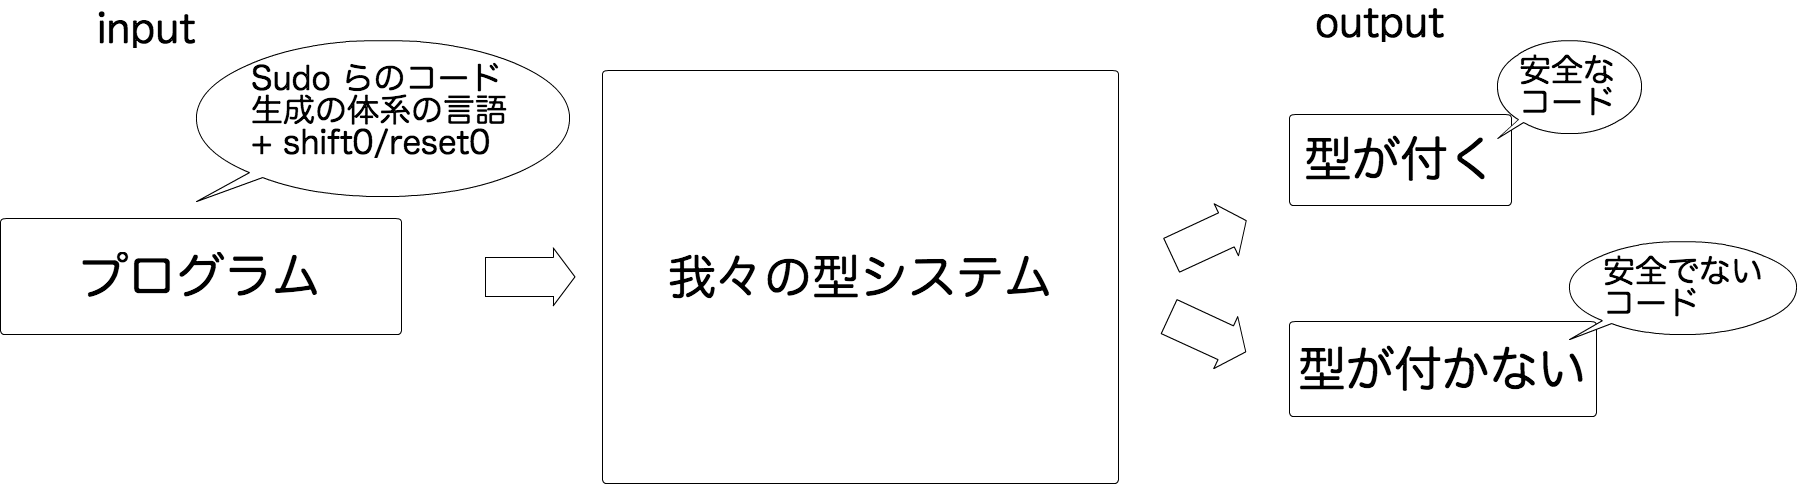
\includegraphics[clip,height=3.2cm]{./img/code_s0r0.png}
    \end{column}
  \end{columns}
\end{frame}



\subsection{コード生成器と生成されるコード}

\begin{frame}
  \center
  \huge{まず表現力について}
\end{frame}

\begin{frame}
  \frametitle{コード生成器と生成されるコード}

  \begin{onlyenv}<1>
    \begin{columns}
      \begin{column}{0.5\textwidth}%% [横幅] 0.2\textwidth = ページ幅の 20 %
        コード生成器
        \begin{align*}
          & \red{...}~ \cfordo{i = 0}{n} \\
          & ~~\red{...}~ \cfordo{j = 0}{m} \\
          & ~~~~\red{...}~ \magenta{\cLet~y=t~\cIn} \\
          & ~~~~~~\red{...}~ (\caryset{\code{a}}{(i,j)}{b[i] + y})
        \end{align*}
      \end{column}
      $\Rightarrow$
      \begin{column}{0.5\textwidth}%% [横幅] 0.2\textwidth = ページ幅の 20 %
        生成されるコード
        \begin{align*}
          & \magenta{\Let ~y ~= ~t ~\In} \\
          & ~~\fordo{i = 0}{n} \\
          & ~~~~\fordo{j = 0}{m} \\
          & ~~~~~~\aryset{a}{i,j}{b[i] + y}
        \end{align*}
      \end{column}
    \end{columns}
  \end{onlyenv}
\end{frame}


% 以降はコード生成器のみの話にしぼって話します

\subsection{多段階let 挿入}

\begin{frame}
  \frametitle{shift0/reset0 による多段階let挿入}
  \begin{onlyenv}<1->
    \begin{align*}
      \Resetz (E[\Shiftz~ k \to e]) &\to e \ksubst{k}{E}
    \end{align*}
  \end{onlyenv}

  \begin{onlyenv}<1>
    コード生成器
    \begin{align*}
      & \red{...}~ \cfordo{i = 0}{n} \\
      & ~~\red{...}~ \cfordo{j = 0}{m} \\
      & ~~~~\red{...}~ \magenta{\cLet~y=t~\cIn} \\
      & ~~~~~~\red{...}~ (\caryset{\code{a}}{(i,j)}{b[i] + y})
    \end{align*}

    \begin{invisibleenv}<1>
      \begin{align*}
        \red{k_1} &= ~~\cfordo{i = 0}{n} \\
        \blue{k_2} &= ~~\cfordo{j = 0}{m} \\
      \end{align*}
    \end{invisibleenv}
  \end{onlyenv}

  \begin{onlyenv}<2>
    コード生成器
    \begin{align*}
      & \red{\Resetz} ~~\cfordo{i = 0}{n} \\
      & ~~\blue{\Resetz} ~~\cfordo{j = 0}{m} \\
      & ~~~~\blue{\Shiftz}~\blue{k_2}~\to~ \red{\Shiftz}~\red{k_1}~\to~ \magenta{\cLet~y=t~\cIn} \\
      & ~~~~~~\red{k_1}~(\blue{k_2}~(\caryset{\code{a}}{(i,j)}{b[i] + y}))
    \end{align*}
    \begin{invisibleenv}<2>
      \begin{align*}
        \red{k_1} &= ~~\cfordo{i = 0}{n} \\
        \blue{k_2} &= ~~\cfordo{j = 0}{m} \\
      \end{align*}
    \end{invisibleenv}
  \end{onlyenv}

  \begin{onlyenv}<3>
    コード生成器
    \begin{align*}
      & \red{\Resetz} ~~\cfordo{i = 0}{n} \\
      & ~~\blue{\Resetz} ~~\cfordo{j = 0}{m} \\
      & ~~~~\blue{\Shiftz}~\blue{k_2}~\to~ \red{\Shiftz}~\red{k_1}~\to~ \magenta{\cLet~y=t~\cIn} \\
      & ~~~~~~\red{k_1}~(\blue{k_2}~(\caryset{\code{a}}{(i,j)}{b[i] + y}))
    \end{align*}
    \begin{align*}
      \red{k_1} &= ~~\cfordo{i = 0}{n} \\
      \blue{k_2} &= ~~\cfordo{j = 0}{m} \\
    \end{align*}
  \end{onlyenv}

  \begin{onlyenv}<4>
    コード生成器
    \begin{align*}
      & \magenta{\cLet~y=t~\cIn} \\
      & ~~\red{k_1}~(\blue{k_2}~(\caryset{\code{a}}{(i,j)}{b[i] + y}))
    \end{align*}
    \begin{align*}
      \red{k_1} &= ~~\cfordo{i = 0}{n} \\
      \blue{k_2} &= ~~\cfordo{j = 0}{m} \\
    \end{align*}
  \end{onlyenv}

  \begin{onlyenv}<5>
    生成されるコード
    \begin{align*}
      & \magenta{\Let ~y ~= ~t ~\In} \\
      & ~~\fordo{i = 0}{n} \\
      & ~~~~\fordo{j = 0}{m} \\
      & ~~~~~~\aryset{a}{i,j}{b[i] + y} \\
    \end{align*}
  \end{onlyenv}
\end{frame}

\begin{frame}
  \center
  \huge{次に安全性}
\end{frame}

\begin{frame}
  \center
  \huge{コード生成前の段階で,安全なコードかどうかを判断する}
\end{frame}

% \begin{frame}
%   \center
%   \huge{安全なコードにのみ型をつけるにはどうすればよいか}
% \end{frame}

\subsection{型システム}

\begin{frame}
  \frametitle{環境識別子 EC によるスコープ表現 [Taha+2003] [Sudo+2014]}
  \begin{center}
    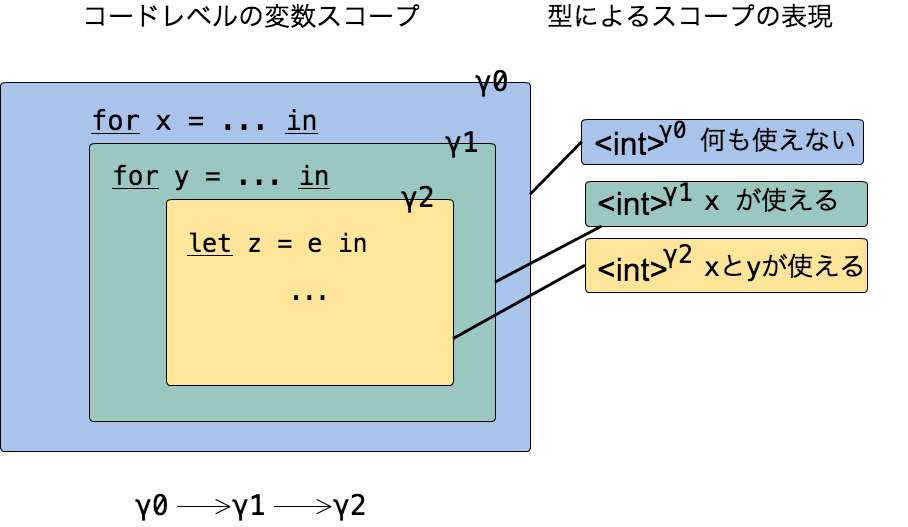
\includegraphics[clip,height=5.7cm]{./img/ec_for.png}
  \end{center}
  \begin{flushright}
    $\gamma_i ... \text{Refined Environment Classifier}$
  \end{flushright}
\end{frame}

\begin{frame}
  \frametitle{ECの洗練化 (本研究)}
  \begin{onlyenv}<1>
    \flushleft
    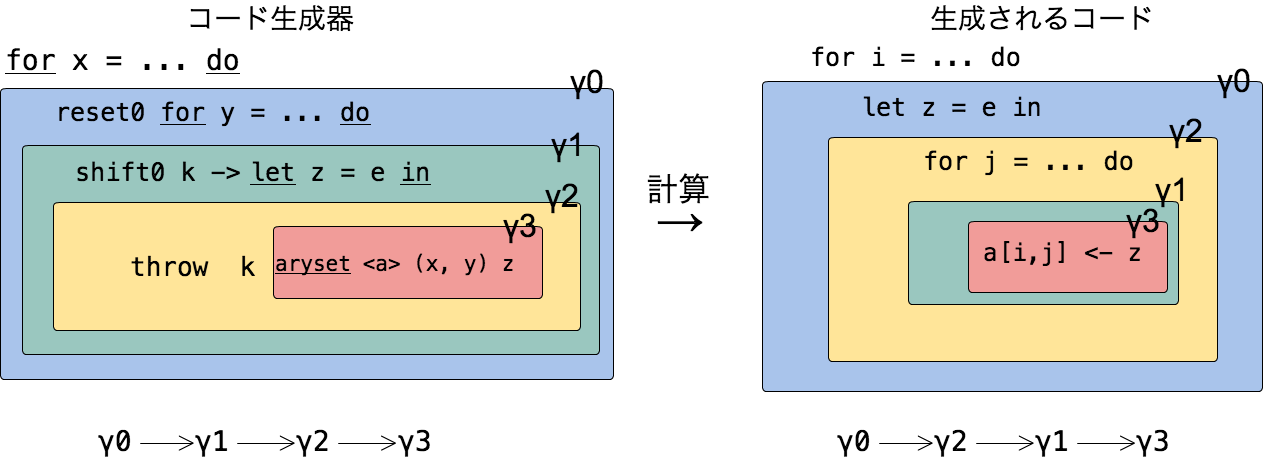
\includegraphics[clip,height=4cm]{./img/ecex.png}
  \end{onlyenv}
\end{frame}

\begin{frame}
  \frametitle{ECの洗練化 (本研究)}
  \begin{onlyenv}<1>
    \begin{center}
      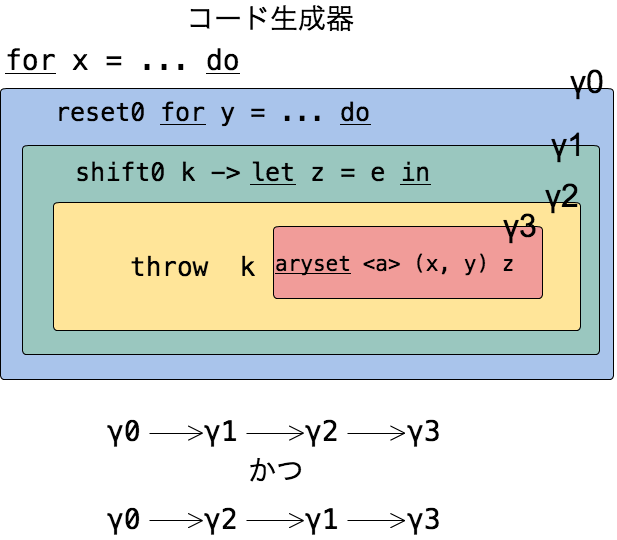
\includegraphics[clip,height=6cm]{./img/ecex_katsu.png}
    \end{center}
  \end{onlyenv}

  \begin{onlyenv}<2>
    \begin{center}
      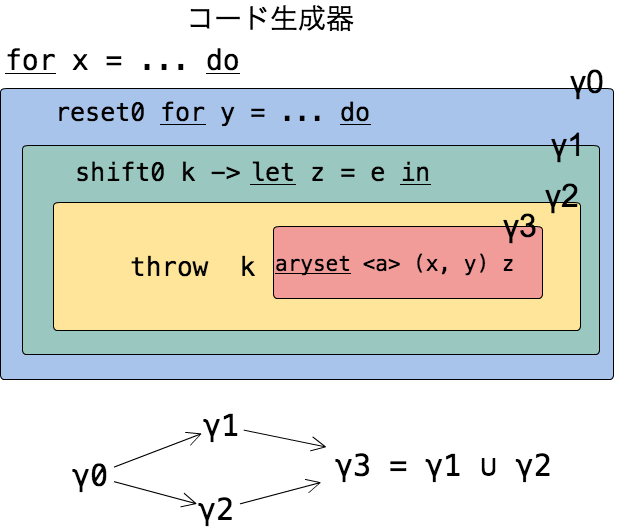
\includegraphics[clip,height=6cm]{./img/ecex_join.png}
    \end{center}
  \end{onlyenv}
\end{frame}


\begin{frame}
  \frametitle{ECのジョイン}
  \flushleft
  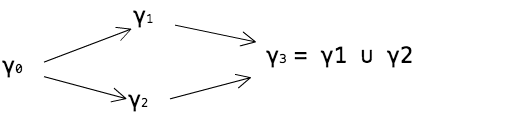
\includegraphics[clip,height=3cm]{./img/ecgraph.png}
  \begin{itemize}
  \item<2-> $\gamma_1$ のコードレベル変数は $\gamma_2$ では使えない
  \item<3-> $\gamma_2$ のコードレベル変数は $\gamma_1$ では使えない
  \item<4-> $\gamma_1, \gamma_2$ のコードレベル変数は $\gamma_3$ で使える
  \item<5->[$\Rightarrow$] Sudoらの体系に $\cup$ を追加
  \end{itemize}
\end{frame}

\begin{frame}[fragile]
  \frametitle{コード生成+shift0/reset0 の型システム (の一部)}
  コードレベルのラムダ抽象:
  \[
    \infer[(\gamma_1~\text{is eigen var})]
    {\Gamma \vdash \cfun{x}{e} : \codeT{t_1\to t_2}{\gamma} ~;~ \sigma}
    {\Gamma,~\gamma_1 \ord \gamma,~x:\codeT{t_1}{\gamma_1} \vdash e
      : \codeT{t_2}{\gamma_1}; \sigma}
  \]

  reset0:
  \[
    \infer{\Gamma \vdash \resetz{e} : \codeT{t}{\gamma} ~;~ \sigma}
    {\Gamma \vdash e : \codeT{t}{\gamma} ~;~ \codeT{t}{\gamma}, \sigma}
  \]

  shift0:
  \[
    \infer{\Gamma \vdash \shiftz{k}{e} : \codeT{t_1}{\gamma_1} ~;~ \codeT{t_0}{\gamma_0},\sigma}
    {\Gamma,~k:\contT{\codeT{t_1}{\gamma_1}}{\codeT{t_0}{\gamma_0}}{\sigma}
      \vdash e : \codeT{t_0}{\gamma_0} ; \sigma
      & \Gamma \models \gamma_1 \ord \gamma_0
    }
  \]

  throw:
  \[
  \infer
  {\Gamma,~k:\contT{\codeT{t_1}{\gamma_1}}{\codeT{t_0}{\gamma_0}}{\sigma}
    \vdash \throw{k}{v} : \codeT{t_0}{\gamma_2} ; \sigma}
  {\Gamma
    \vdash v : \codeT{t_1}{\gamma_1 \cup \gamma_2} ; \sigma
    & \Gamma \models \gamma_2 \ord \gamma_0
  }
\]

\end{frame}


%%% Local Variables:
%%% mode: japanese-latex
%%% TeX-master: "slide"
%%% End:
